

\tikzset{every picture/.style={line width=0.75pt}} %set default line width to 0.75pt        

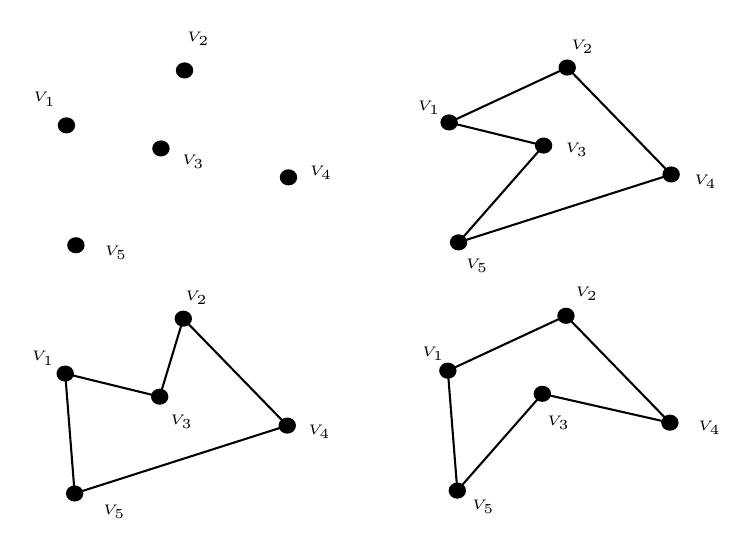
\begin{tikzpicture}[x=0.75pt,y=0.75pt,yscale=-1,xscale=1]
%uncomment if require: \path (0,300); %set diagram left start at 0, and has height of 300

%Shape: Ellipse [id:dp0903854075610232] 
\draw  [fill={rgb, 255:red, 0; green, 0; blue, 0 }  ,fill opacity=1 ] (173.3,63.55) .. controls (173.3,61.69) and (174.95,60.18) .. (176.98,60.18) .. controls (179.01,60.18) and (180.66,61.69) .. (180.66,63.55) .. controls (180.66,65.42) and (179.01,66.93) .. (176.98,66.93) .. controls (174.95,66.93) and (173.3,65.42) .. (173.3,63.55) -- cycle ;
%Shape: Ellipse [id:dp3184910134932345] 
\draw  [fill={rgb, 255:red, 0; green, 0; blue, 0 }  ,fill opacity=1 ] (177.85,121.32) .. controls (177.85,119.46) and (179.5,117.95) .. (181.53,117.95) .. controls (183.56,117.95) and (185.21,119.46) .. (185.21,121.32) .. controls (185.21,123.19) and (183.56,124.7) .. (181.53,124.7) .. controls (179.5,124.7) and (177.85,123.19) .. (177.85,121.32) -- cycle ;
%Shape: Ellipse [id:dp5872048719836919] 
\draw  [fill={rgb, 255:red, 0; green, 0; blue, 0 }  ,fill opacity=1 ] (280.28,88.61) .. controls (280.28,86.75) and (281.92,85.23) .. (283.96,85.23) .. controls (285.99,85.23) and (287.64,86.75) .. (287.64,88.61) .. controls (287.64,90.47) and (285.99,91.99) .. (283.96,91.99) .. controls (281.92,91.99) and (280.28,90.47) .. (280.28,88.61) -- cycle ;
%Shape: Ellipse [id:dp7591641248768922] 
\draw  [fill={rgb, 255:red, 0; green, 0; blue, 0 }  ,fill opacity=1 ] (230.2,37.1) .. controls (230.2,35.24) and (231.85,33.73) .. (233.88,33.73) .. controls (235.91,33.73) and (237.56,35.24) .. (237.56,37.1) .. controls (237.56,38.97) and (235.91,40.48) .. (233.88,40.48) .. controls (231.85,40.48) and (230.2,38.97) .. (230.2,37.1) -- cycle ;
%Shape: Ellipse [id:dp7762987079639629] 
\draw  [fill={rgb, 255:red, 0; green, 0; blue, 0 }  ,fill opacity=1 ] (218.82,74.69) .. controls (218.82,72.82) and (220.47,71.31) .. (222.5,71.31) .. controls (224.53,71.31) and (226.18,72.82) .. (226.18,74.69) .. controls (226.18,76.55) and (224.53,78.06) .. (222.5,78.06) .. controls (220.47,78.06) and (218.82,76.55) .. (218.82,74.69) -- cycle ;
%Shape: Ellipse [id:dp7626801331888498] 
\draw  [fill={rgb, 255:red, 0; green, 0; blue, 0 }  ,fill opacity=1 ] (357.66,62.16) .. controls (357.66,60.29) and (359.31,58.78) .. (361.34,58.78) .. controls (363.38,58.78) and (365.02,60.29) .. (365.02,62.16) .. controls (365.02,64.02) and (363.38,65.54) .. (361.34,65.54) .. controls (359.31,65.54) and (357.66,64.02) .. (357.66,62.16) -- cycle ;
%Shape: Ellipse [id:dp6435093773617909] 
\draw  [fill={rgb, 255:red, 0; green, 0; blue, 0 }  ,fill opacity=1 ] (362.22,119.93) .. controls (362.22,118.07) and (363.86,116.56) .. (365.9,116.56) .. controls (367.93,116.56) and (369.58,118.07) .. (369.58,119.93) .. controls (369.58,121.8) and (367.93,123.31) .. (365.9,123.31) .. controls (363.86,123.31) and (362.22,121.8) .. (362.22,119.93) -- cycle ;
%Shape: Ellipse [id:dp23520259436348545] 
\draw  [fill={rgb, 255:red, 0; green, 0; blue, 0 }  ,fill opacity=1 ] (464.64,87.22) .. controls (464.64,85.35) and (466.29,83.84) .. (468.32,83.84) .. controls (470.35,83.84) and (472,85.35) .. (472,87.22) .. controls (472,89.08) and (470.35,90.59) .. (468.32,90.59) .. controls (466.29,90.59) and (464.64,89.08) .. (464.64,87.22) -- cycle ;
%Shape: Ellipse [id:dp5139999912619062] 
\draw  [fill={rgb, 255:red, 0; green, 0; blue, 0 }  ,fill opacity=1 ] (414.57,35.71) .. controls (414.57,33.84) and (416.21,32.33) .. (418.25,32.33) .. controls (420.28,32.33) and (421.93,33.84) .. (421.93,35.71) .. controls (421.93,37.57) and (420.28,39.09) .. (418.25,39.09) .. controls (416.21,39.09) and (414.57,37.57) .. (414.57,35.71) -- cycle ;
%Shape: Ellipse [id:dp9128853181814609] 
\draw  [fill={rgb, 255:red, 0; green, 0; blue, 0 }  ,fill opacity=1 ] (403.19,73.3) .. controls (403.19,71.43) and (404.83,69.92) .. (406.87,69.92) .. controls (408.9,69.92) and (410.55,71.43) .. (410.55,73.3) .. controls (410.55,75.16) and (408.9,76.67) .. (406.87,76.67) .. controls (404.83,76.67) and (403.19,75.16) .. (403.19,73.3) -- cycle ;
%Straight Lines [id:da45150527483296576] 
\draw    (361.34,62.16) -- (406.87,73.3) ;
%Straight Lines [id:da030554361443556277] 
\draw    (361.34,62.16) -- (418.25,35.71) ;
%Straight Lines [id:da1930137132355716] 
\draw    (418.25,35.71) -- (468.32,87.22) ;
%Straight Lines [id:da9231067498266883] 
\draw    (365.9,119.93) -- (468.32,87.22) ;
%Shape: Ellipse [id:dp4319239618273387] 
\draw  [fill={rgb, 255:red, 0; green, 0; blue, 0 }  ,fill opacity=1 ] (172.7,183.15) .. controls (172.7,181.29) and (174.35,179.78) .. (176.38,179.78) .. controls (178.41,179.78) and (180.06,181.29) .. (180.06,183.15) .. controls (180.06,185.02) and (178.41,186.53) .. (176.38,186.53) .. controls (174.35,186.53) and (172.7,185.02) .. (172.7,183.15) -- cycle ;
%Shape: Ellipse [id:dp7164128195056259] 
\draw  [fill={rgb, 255:red, 0; green, 0; blue, 0 }  ,fill opacity=1 ] (177.25,240.92) .. controls (177.25,239.06) and (178.9,237.55) .. (180.93,237.55) .. controls (182.96,237.55) and (184.61,239.06) .. (184.61,240.92) .. controls (184.61,242.79) and (182.96,244.3) .. (180.93,244.3) .. controls (178.9,244.3) and (177.25,242.79) .. (177.25,240.92) -- cycle ;
%Shape: Ellipse [id:dp9814273885878707] 
\draw  [fill={rgb, 255:red, 0; green, 0; blue, 0 }  ,fill opacity=1 ] (279.68,208.21) .. controls (279.68,206.35) and (281.32,204.83) .. (283.36,204.83) .. controls (285.39,204.83) and (287.04,206.35) .. (287.04,208.21) .. controls (287.04,210.07) and (285.39,211.59) .. (283.36,211.59) .. controls (281.32,211.59) and (279.68,210.07) .. (279.68,208.21) -- cycle ;
%Shape: Ellipse [id:dp9377208715905136] 
\draw  [fill={rgb, 255:red, 0; green, 0; blue, 0 }  ,fill opacity=1 ] (229.6,156.7) .. controls (229.6,154.84) and (231.25,153.33) .. (233.28,153.33) .. controls (235.31,153.33) and (236.96,154.84) .. (236.96,156.7) .. controls (236.96,158.57) and (235.31,160.08) .. (233.28,160.08) .. controls (231.25,160.08) and (229.6,158.57) .. (229.6,156.7) -- cycle ;
%Shape: Ellipse [id:dp30420219582704955] 
\draw  [fill={rgb, 255:red, 0; green, 0; blue, 0 }  ,fill opacity=1 ] (218.22,194.29) .. controls (218.22,192.42) and (219.87,190.91) .. (221.9,190.91) .. controls (223.93,190.91) and (225.58,192.42) .. (225.58,194.29) .. controls (225.58,196.15) and (223.93,197.66) .. (221.9,197.66) .. controls (219.87,197.66) and (218.22,196.15) .. (218.22,194.29) -- cycle ;
%Shape: Ellipse [id:dp6697232002405218] 
\draw  [fill={rgb, 255:red, 0; green, 0; blue, 0 }  ,fill opacity=1 ] (357.06,181.76) .. controls (357.06,179.89) and (358.71,178.38) .. (360.74,178.38) .. controls (362.78,178.38) and (364.42,179.89) .. (364.42,181.76) .. controls (364.42,183.62) and (362.78,185.14) .. (360.74,185.14) .. controls (358.71,185.14) and (357.06,183.62) .. (357.06,181.76) -- cycle ;
%Shape: Ellipse [id:dp3942573514201133] 
\draw  [fill={rgb, 255:red, 0; green, 0; blue, 0 }  ,fill opacity=1 ] (361.62,239.53) .. controls (361.62,237.67) and (363.26,236.16) .. (365.3,236.16) .. controls (367.33,236.16) and (368.98,237.67) .. (368.98,239.53) .. controls (368.98,241.4) and (367.33,242.91) .. (365.3,242.91) .. controls (363.26,242.91) and (361.62,241.4) .. (361.62,239.53) -- cycle ;
%Shape: Ellipse [id:dp991801762708085] 
\draw  [fill={rgb, 255:red, 0; green, 0; blue, 0 }  ,fill opacity=1 ] (464.04,206.82) .. controls (464.04,204.95) and (465.69,203.44) .. (467.72,203.44) .. controls (469.75,203.44) and (471.4,204.95) .. (471.4,206.82) .. controls (471.4,208.68) and (469.75,210.19) .. (467.72,210.19) .. controls (465.69,210.19) and (464.04,208.68) .. (464.04,206.82) -- cycle ;
%Shape: Ellipse [id:dp22587871703179985] 
\draw  [fill={rgb, 255:red, 0; green, 0; blue, 0 }  ,fill opacity=1 ] (413.97,155.31) .. controls (413.97,153.44) and (415.61,151.93) .. (417.65,151.93) .. controls (419.68,151.93) and (421.33,153.44) .. (421.33,155.31) .. controls (421.33,157.17) and (419.68,158.69) .. (417.65,158.69) .. controls (415.61,158.69) and (413.97,157.17) .. (413.97,155.31) -- cycle ;
%Shape: Ellipse [id:dp5394518773608862] 
\draw  [fill={rgb, 255:red, 0; green, 0; blue, 0 }  ,fill opacity=1 ] (402.59,192.9) .. controls (402.59,191.03) and (404.23,189.52) .. (406.27,189.52) .. controls (408.3,189.52) and (409.95,191.03) .. (409.95,192.9) .. controls (409.95,194.76) and (408.3,196.27) .. (406.27,196.27) .. controls (404.23,196.27) and (402.59,194.76) .. (402.59,192.9) -- cycle ;
%Straight Lines [id:da30052767091565935] 
\draw    (176.38,183.15) -- (180.93,240.92) ;
%Straight Lines [id:da045332267906341595] 
\draw    (176.38,183.15) -- (221.9,194.29) ;
%Straight Lines [id:da006754746917110088] 
\draw    (233.28,156.7) -- (283.36,208.21) ;
%Straight Lines [id:da9808534458563097] 
\draw    (283.36,208.21) -- (180.93,240.92) ;
%Straight Lines [id:da7788956384610358] 
\draw    (360.74,181.76) -- (365.3,239.53) ;
%Straight Lines [id:da24525394239037623] 
\draw    (360.74,181.76) -- (417.65,155.31) ;
%Straight Lines [id:da15224280273103452] 
\draw    (417.65,155.31) -- (467.72,206.82) ;
%Straight Lines [id:da7264188286372529] 
\draw    (365.3,239.53) -- (406.27,192.9) ;
%Straight Lines [id:da18718151665886473] 
\draw    (406.87,73.3) -- (365.9,119.93) ;
%Straight Lines [id:da8596127984251889] 
\draw    (233.28,156.7) -- (221.9,194.29) ;
%Straight Lines [id:da67879921706725] 
\draw    (467.72,206.82) -- (406.27,192.9) ;

% Text Node
\draw (159.6,46.2) node [anchor=north west][inner sep=0.75pt]  [font=\tiny] [align=left] {$\displaystyle {\displaystyle V_{1}}$};
% Text Node
\draw (194,120.2) node [anchor=north west][inner sep=0.75pt]  [font=\tiny] [align=left] {$\displaystyle {\displaystyle V_{5}}$};
% Text Node
\draw (231.2,76.2) node [anchor=north west][inner sep=0.75pt]  [font=\tiny] [align=left] {$\displaystyle {\displaystyle V_{3}}$};
% Text Node
\draw (292.8,81.8) node [anchor=north west][inner sep=0.75pt]  [font=\tiny] [align=left] {$\displaystyle {\displaystyle V_{4}}$};
% Text Node
\draw (233.6,17) node [anchor=north west][inner sep=0.75pt]  [font=\tiny] [align=left] {$\displaystyle {\displaystyle V_{2}}$};
% Text Node
\draw (344.8,50.2) node [anchor=north west][inner sep=0.75pt]  [font=\tiny] [align=left] {$\displaystyle {\displaystyle V_{1}}$};
% Text Node
\draw (367.9,126.31) node [anchor=north west][inner sep=0.75pt]  [font=\tiny] [align=left] {$\displaystyle {\displaystyle V_{5}}$};
% Text Node
\draw (416,70.6) node [anchor=north west][inner sep=0.75pt]  [font=\tiny] [align=left] {$\displaystyle {\displaystyle V_{3}}$};
% Text Node
\draw (478,85.8) node [anchor=north west][inner sep=0.75pt]  [font=\tiny] [align=left] {$\displaystyle {\displaystyle V_{4}}$};
% Text Node
\draw (418.8,21) node [anchor=north west][inner sep=0.75pt]  [font=\tiny] [align=left] {$\displaystyle {\displaystyle V_{2}}$};
% Text Node
\draw (346.8,169) node [anchor=north west][inner sep=0.75pt]  [font=\tiny] [align=left] {$\displaystyle {\displaystyle V_{1}}$};
% Text Node
\draw (370.98,242.53) node [anchor=north west][inner sep=0.75pt]  [font=\tiny] [align=left] {$\displaystyle {\displaystyle V_{5}}$};
% Text Node
\draw (407.2,202.2) node [anchor=north west][inner sep=0.75pt]  [font=\tiny] [align=left] {$\displaystyle {\displaystyle V_{3}}$};
% Text Node
\draw (480,204.6) node [anchor=north west][inner sep=0.75pt]  [font=\tiny] [align=left] {$\displaystyle {\displaystyle V_{4}}$};
% Text Node
\draw (420.8,139.8) node [anchor=north west][inner sep=0.75pt]  [font=\tiny] [align=left] {$\displaystyle {\displaystyle V_{2}}$};
% Text Node
\draw (158.8,171) node [anchor=north west][inner sep=0.75pt]  [font=\tiny] [align=left] {$\displaystyle {\displaystyle V_{1}}$};
% Text Node
\draw (193.2,245) node [anchor=north west][inner sep=0.75pt]  [font=\tiny] [align=left] {$\displaystyle {\displaystyle V_{5}}$};
% Text Node
\draw (225.6,201.8) node [anchor=north west][inner sep=0.75pt]  [font=\tiny] [align=left] {$\displaystyle {\displaystyle V_{3}}$};
% Text Node
\draw (292,206.6) node [anchor=north west][inner sep=0.75pt]  [font=\tiny] [align=left] {$\displaystyle {\displaystyle V_{4}}$};
% Text Node
\draw (232.8,141.8) node [anchor=north west][inner sep=0.75pt]  [font=\tiny] [align=left] {$\displaystyle {\displaystyle V_{2}}$};


\end{tikzpicture}
